\section{Systemarkitektur}
\label{chap:systemarkitektur}

Til at dokumentere systemarkitekturen er der anvendt SysML  til visualisering af de hardware blokke der indgår i systemet. UML diagrammer er anvendt til at uddybe software og hvordan softwaren er designet i projektet. Til supplering af UML diagrammer er n+1 modellen anvendt. N+1 modellen er en udviklingsmodel til software, som benytter sig af forskellige views til at illustrere og informere hvordan systemet er designet og implementeret.
 
\subsection{Blokbeskrivelser}
Det overordnede bdd på figur \ref{fig:bdd_asd} viser hvilke blokke systemet består af, samt hvilke parts blokkene indeholder.

\begin{figure}[H]
	\centering
	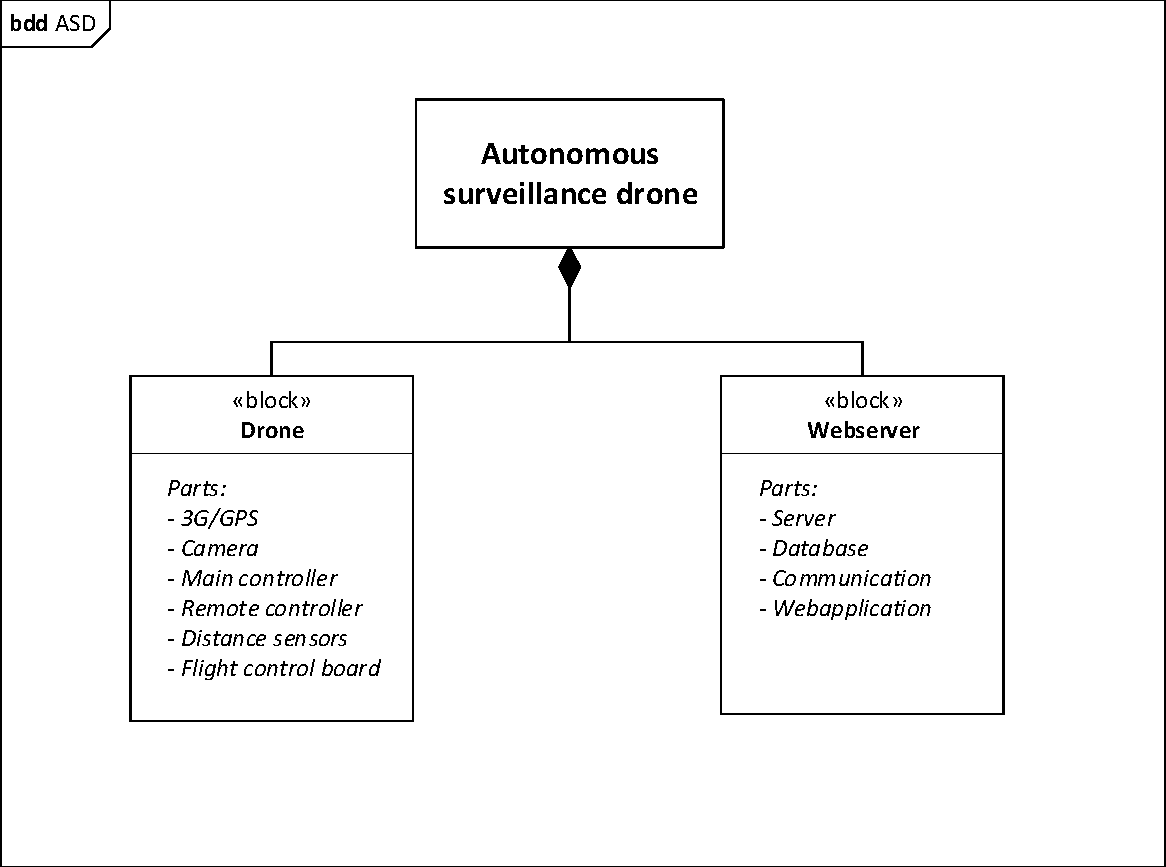
\includegraphics[width=0.80\textwidth]{Billeder/Projektbeskrivelse/bdd_overordnet.pdf}
	\caption{Overordnet bdd for systemet}
	\label{fig:bdd_asd}
\end{figure}

\textbf{Drone} \\
Drone blokken indeholder alt funktionalitet til dronen. Yderligere beskrivelse af de interne forbindelser imellem alle parts er beskrevet i dokumentationens systemarkitektur og design.

\textbf{Webserver} \\
Webserver blokken indeholder de hardware moduler der anvendes til server og webapplikationen. 


\subsection{Interne forbindelser}

Det overordnede ibd på figur \ref{fig:ibd_asd} beskriver hvorledes de forskellige blokke kommunikerer samt hvilken type signal, der anvendes.

\begin{figure}[H]
	\centering
	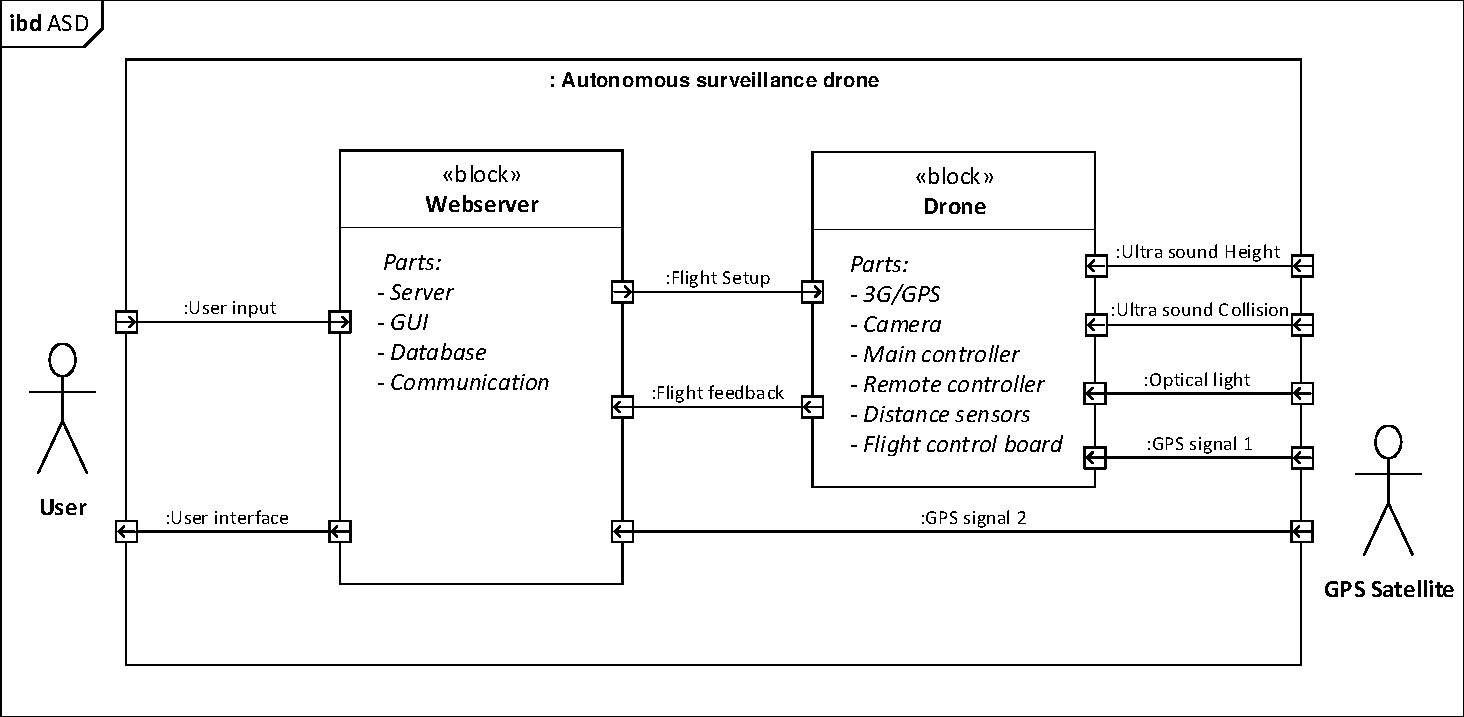
\includegraphics[width=1\textwidth]{Billeder/Projektbeskrivelse/ibd1_overordnet.pdf}
	\caption{Overordnet ibd for systemet}
	\label{fig:ibd_asd}
\end{figure}

\subsection{Pakke diagram}

For at definere hvilke

\begin{figure}[H]
	\centering
	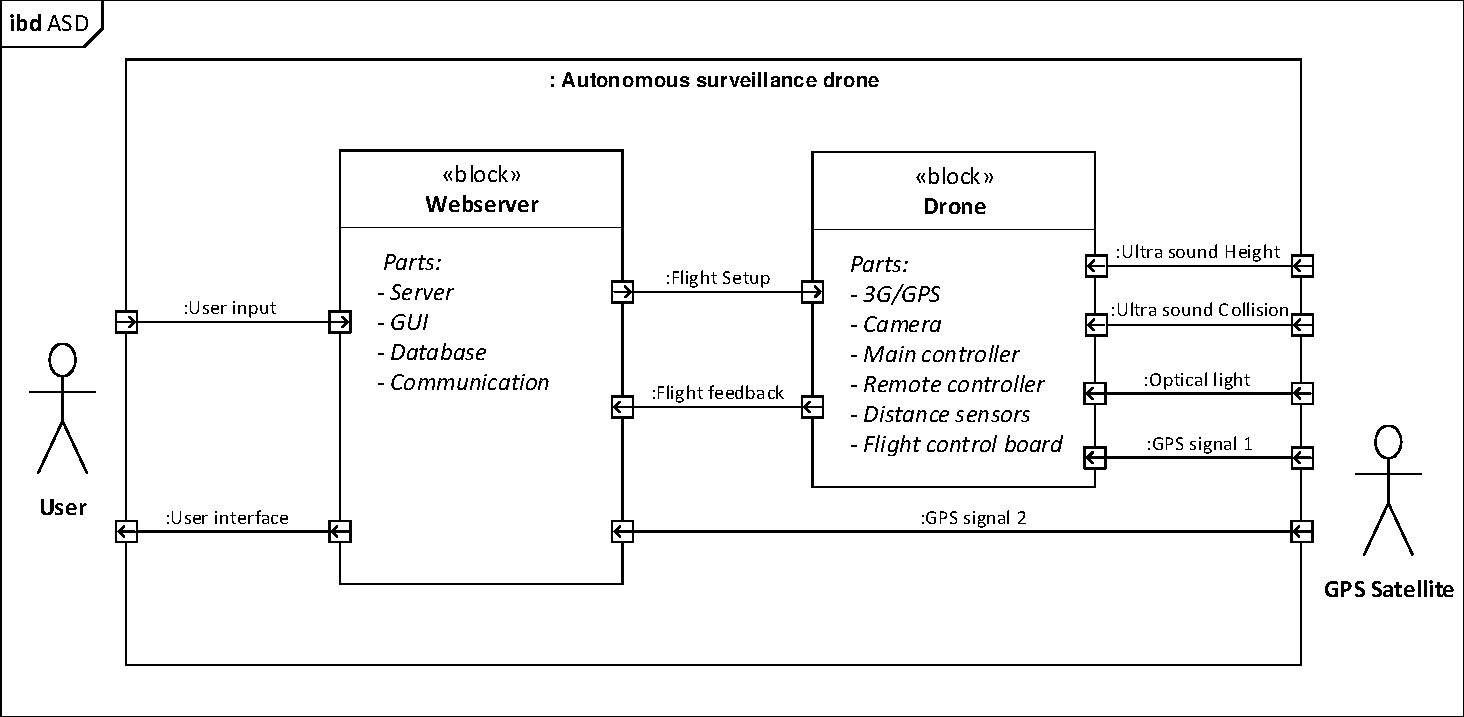
\includegraphics[width=1\textwidth]{Billeder/Projektbeskrivelse/ibd1_overordnet.pdf}
	\caption{Overordnet ibd for systemet}
	\label{fig:ibd_asd}
\end{figure}